\section{Soluzione Proposta}

\begin{frame}{Progettazione}
Il funzionamento di un Vulnerability Scanner può essere riassunto in \textbf{cinque fasi}
\vspace{0.2cm}
\begin{figure}
    \centering
    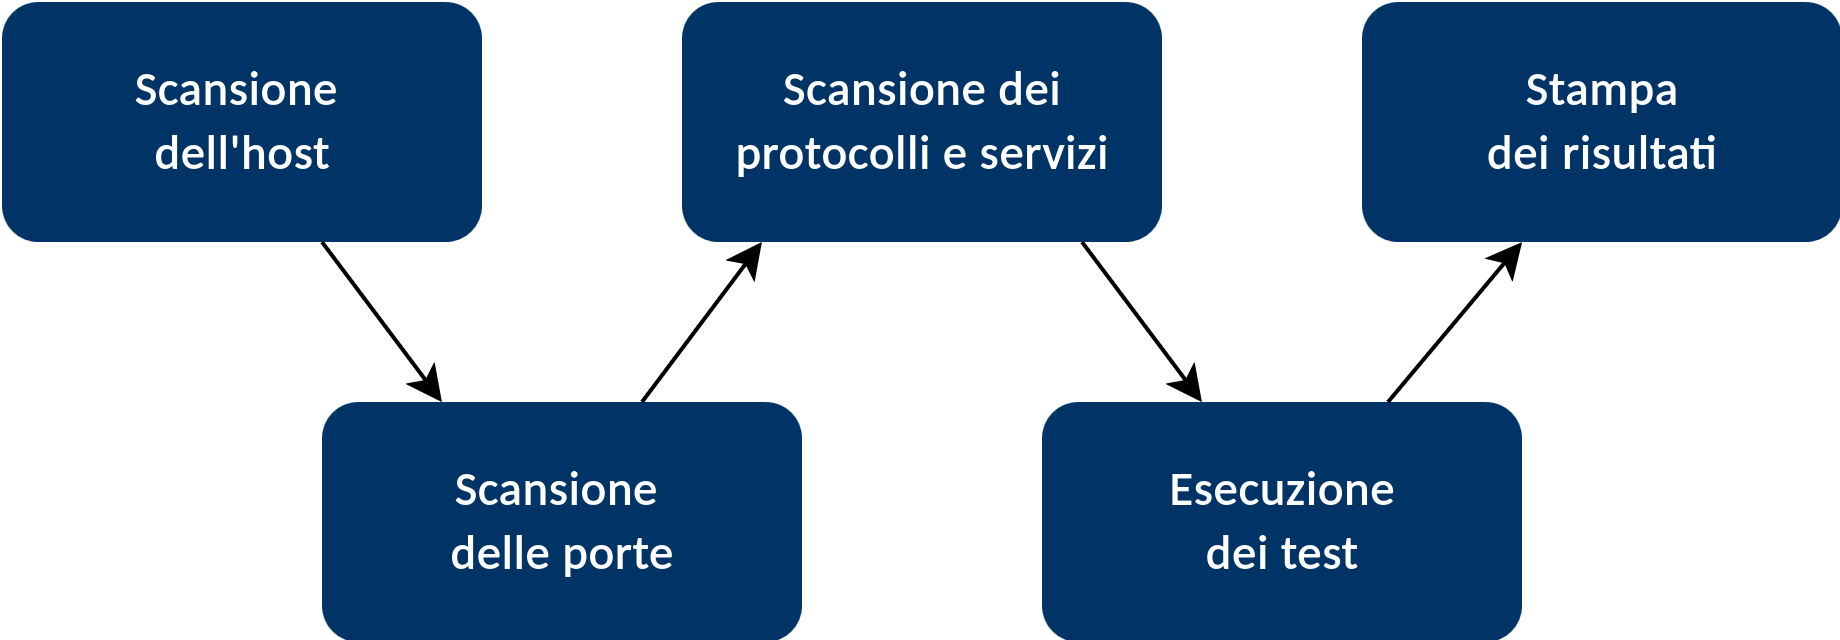
\includegraphics[width=12cm]{assets/mio/Fasi_scan.png}
\end{figure}
\end{frame}

%=======================================================================

%\begin{frame}{Implementazione}
%L'implementazione dell'applicativo è suddiviso in due moduli principali: \textbf{agent} e \textbf{utils}
%\vspace{0.4cm}
%    \begin{columns} 
%    \begin{column}{0.5\textwidth}
%    \begin{figure}
%    \centering
%    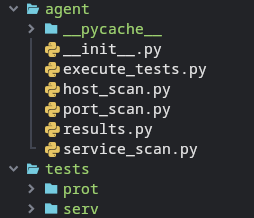
\includegraphics[width=5cm]{assets/mio/File1.png}
%    \end{figure}
%    \end{column}
%    \begin{column}{0.5\textwidth}
%    \begin{figure}
%    \centering
%    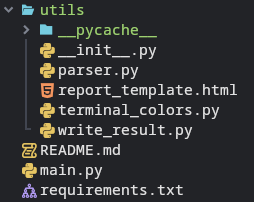
\includegraphics[width=5cm]{assets/mio/File2.png}
%    \end{figure}
%    \end{column}
%    \end{columns}
%\end{frame}

%=======================================================================

\begin{frame}[fragile]{Implementazione}
\centering
\textbf{Manuale di utilizzo}
\begin{lstlisting}[style=statale, basicstyle=\tiny]
usage: main.py [-h] [-v] [-nt] [-hs HOST_SCAN] [-ps PORT_SCAN] ports host

Agent for Advanced Network Protocol Verification. This program needs sudo privileges to run.

positional arguments:
  ports                 Single port [x], multiple ports [x,y,z], port range [x:y] to scan or all ports [all]
  host                  Host to scan using ipv4 address

options:
  -h, --help            Show this help message and exit
  -v, --verbose         Increase output verbosity
  -nt, --no_tests       Scans the target for services but doesn't execute a vulnerability scan
  -hs, --host_scan HOST_SCAN
                        Host scan to execute: [p]ing, [s]yn, [a]ck, [u]dp (ping scan will be used by default)
  -ps, --port_scan PORT_SCAN
                        Port scan to execute: [c]onnect, [s]yn, [f]in, [n]ull, [x]mas, [u]dp (connect scan 
                        will be used by default)
\end{lstlisting}
\end{frame}

%=======================================================================

\begin{frame}[fragile]{Scansione delle Porte}
\begin{columns}
\begin{column}{0.5\textwidth}
\centering
\textbf{Scansione di tipo SYN}
\begin{lstlisting}[style=statalepython, basicstyle=\tiny]
packet = IP(dst=self.ip) / TCP(dport=port, flags="S")
res = sr1(packet, timeout=3, verbose=0)

if res is None or (
    res.sprintf("%ICMP.type%") == 3
    and res.sprintf("%ICMP.code%") in [1, 2, 3, 9, 10, 13]
):
    self.ports[port] = "filtered"

else:
    flag_res = res.sprintf("%TCP.flags%")

    if flag_res == "RA":
        self.ports[port] = "closed"
    elif flag_res == "SA":
        self.ports[port] = "open"
\end{lstlisting}
\end{column}
\begin{column}{0.5\textwidth}
\textbf{Funzionamento generico}:
\begin{itemize}
    \item \textbf{Invio di pacchetti} formattati in modo specifico
    \item \textbf{Analisi} dei contenuti delle \textbf{risposte}
    \item Definizione dello \textbf{stato delle porte}
\end{itemize}
\end{column}
\end{columns}
\end{frame}


%=======================================================================

\begin{frame}[fragile]{Scansione di Protocolli e Servizi}
\begin{columns}
\begin{column}{0.5\textwidth}
\centering
\textbf{Scansione del protocollo HTTP}
\begin{lstlisting}[style=statalepython, basicstyle=\tiny]
try:
    # Tries to establish a connection using HTTP
    conn = HTTPConnection(url.netloc, timeout=3)
    conn.request("HEAD", url.path)
    res = conn.getresponse()

    banner = res.headers["server"]
    if banner is None:
        banner = "undefined"

    service["port"] = port
    service["protocol"] = "HTTP"
    service["service"] = banner

    self.services.append(service)

except Exception:
    pass
\end{lstlisting}
\end{column}
\begin{column}{0.5\textwidth}
\textbf{Funzionamento generico}:
\begin{itemize}
    \item \textbf{Connessione} alla porta utilizzando librerie specifiche dei protocolli
    \item Si tenta il \textbf{recupero del banner} del servizio
    \item Le \textbf{informazioni} ottenute vengono \textbf{salvate}
\end{itemize}
Un protocollo viene \textbf{individuato correttamente} solo quando la connessione alla porta tramite librerie \textbf{non genera errori}
\end{column}
\end{columns}
\end{frame}

%=======================================================================

\begin{frame}[fragile]{File JSON di Test}
\begin{columns}
\begin{column}{0.5\textwidth}
\centering
\textbf{Test per i protocolli}
\begin{lstlisting}[style=statale, basicstyle=\tiny]
  "vulns": {
    "ANONYMOUS LOGIN ENABLED" :{
      "description": "Anonymous login is enabled...",
      "send": "\n~~USER anonymous\n~~PASS\n",
      "recv": "230",
      "severity": "high"
    }
  },
  "login": {
    "send_str": "\n~~USER _username_\n~~PASS _password_\n",
    "recv_str": "230 Login successful."
  },
  "auth_vulns": {
    "BOUNCE ATTACK": {
      "description": "If not correctly configured...",
      "send": "PORT\n",
      "not_recv": "500",
      "severity": "medium"
    }
  },
  "serv_names": [ "vsftpd" ]
\end{lstlisting}
\end{column}
\begin{column}{0.5\textwidth}
\centering
\textbf{Test per i servizi}
\begin{lstlisting}[style=statale, basicstyle=\tiny]
  "vulns": {
    "BACKDOOR COMMAND EXECUTION": {
      "description": "Allows users to leverage a backdoor to make a command execution.",
      "send": "\n~~USER X:)\n~~PASS X\n~~id\n",
      "not_recv": "530",
      "severity": "high"
    }
  },
  "login": {},
  "auth_vulns": {},
  "vuln_serv_version": {
    "2.3.4": ["https://www.cve.org/CVERecord?id=CVE-2011-2523"],
    "3.0.2": ["https://www.cve.org/CVERecord?id=CVE-2015-1419"]
  }
\end{lstlisting}
\end{column}
\end{columns}
\end{frame}

%=======================================================================

\begin{frame}[fragile]{Esecuzione dei Test}
\begin{columns}
\begin{column}{0.55\textwidth}
\begin{lstlisting}[style=statalepython, basicstyle=\tiny]
sock = socket.socket(socket.AF_INET, socket.SOCK_STREAM)
sock.settimeout(5)
sock.connect((ip, port))

for message in login_list:
    sock.send(message.encode())

for send in send_list:
    sock.send(send.encode())
    res = sock.recv(1024)

if (
    recv is not None
    and re.search(recv, res.decode())
    or not_recv is not None
    and not re.search(not_recv, res.decode())
):
    vuln = {}
    vuln["name"] = name
    vuln["service"] = service
    vuln["description"] = info["description"]
    vuln["severity"] = info["severity"]
    return vuln
\end{lstlisting}
\end{column}
\begin{column}{0.45\textwidth}
\textbf{Funzionamento}:
\begin{itemize}
    \item \textbf{Stabilire una connessione} normale o con SSL/TLS verso la porta
    \item \textbf{L'utente viene autenticato} se sono state fornite delle credenziali
    \item \textbf{Invio in sequenza dei comandi} recuperati dal file JSON
    \item \textbf{Analisi del messaggio ricevuto} per identificare la presenza o meno di vulnerabilità
\end{itemize}
\end{column}
\end{columns}
\end{frame}

%=======================================================================

\begin{frame}[fragile]{Altri Test Svolti}
\textbf{Test autenticati}
\begin{lstlisting}[style=statalepython, basicstyle=\tiny]
username = input()
password = getpass.getpass(f"{prot} - {service} password: ")
if username == "" and password == "":
    login_list = []
    return login_list
else:
    login_str = login["send_str"].replace("_username_", username)
    login_str = login_str.replace("_password_", password)

login_list = login_str.split("~~")
for message in login_list:
    sock.send(message.encode())
    res = sock.recv(1024)
\end{lstlisting}
\begin{columns}
\begin{column}{0.5\textwidth}
\textbf{Test versione del servizio}
\begin{lstlisting}[style=statalepython, basicstyle=\tiny]
for version, cve in vuln_serv_version.items():
    if version in service:
        results.unsafe_ver = True
        results.unsafe_ver_cve = cve
\end{lstlisting}
\end{column}
\begin{column}{0.5\textwidth}
\textbf{Test versione SSL/TLS}
\begin{lstlisting}[style=statalepython, basicstyle=\tiny]
if not ("TLSv1.3" in service or "TLSv1.2" in service):
    results.unsafe_tls = True
\end{lstlisting}
\end{column}
\end{columns}

\end{frame}